% --------------------------------------------------------------
% 
% Should be compiled by XeLatex
% 
% --------------------------------------------------------------
 
\documentclass[12pt]{article}
\usepackage[noindent]{ctex}
\usepackage{xeCJK}
\usepackage[margin=1in]{geometry} 
\usepackage{amsmath,amsthm,amssymb}
\usepackage[margin=1in]{geometry} 
\usepackage{amsmath,amsthm,amssymb}
\usepackage[english]{babel} %Castellanización
%\usepackage[T1]{fontenc} %escribe lo del teclado
\usepackage[utf8]{inputenc} %Reconoce algunos símbolos
\usepackage{lmodern} %optimiza algunas fuentes
\usepackage{graphicx}
\graphicspath{ {images/} }
\usepackage{hyperref} % Uso de links
\usepackage{url}
\usepackage{color,xcolor}
\definecolor{steelblue}{RGB}{10, 80, 130}
\definecolor{indianred}{RGB}{185, 72, 72}
\definecolor{forestgreen}{RGB}{4, 69, 4}
\definecolor{ans}{RGB}{67, 92, 114}
\definecolor{gold}{RGB}{198, 161, 0}
\newcommand{\HRule}{\rule{\linewidth}{0.5mm}}
\newcommand{\N}{\mathbb{N}}
\newcommand{\Z}{\mathbb{Z}}
 
 \if0
\newenvironment{theorem}[2][Theorem]{\begin{trivlist}
\item[\hskip \labelsep {\bfseries #1}\hskip \labelsep {\bfseries #2.}]}{\end{trivlist}}
\newenvironment{lemma}[2][Lemma]{\begin{trivlist}
\item[\hskip \labelsep {\bfseries #1}\hskip \labelsep {\bfseries #2.}]}{\end{trivlist}}
\newenvironment{exercise}[2][Exercise]{\begin{trivlist}
\item[\hskip \labelsep {\bfseries #1}\hskip \labelsep {\bfseries #2.}]}{\end{trivlist}}
\newenvironment{problem}[2][Problem]{\begin{trivlist}
\item[\hskip \labelsep {\bfseries #1}\hskip \labelsep {\bfseries #2.}]}{\end{trivlist}}
\newenvironment{question}[2][Question]{\begin{trivlist}
\item[\hskip \labelsep {\bfseries #1}\hskip \labelsep {\bfseries #2.}]}{\end{trivlist}}
\newenvironment{corollary}[2][Corollary]{\begin{trivlist}
\item[\hskip \labelsep {\bfseries #1}\hskip \labelsep {\bfseries #2.}]}{\end{trivlist}}
\fi

\newenvironment{solution}{\begin{proof}[Solution]}{\end{proof}}
 
\begin{document}
 
% --------------------------------------------------------------
%                         Should be compiled by XeLatex
% --------------------------------------------------------------
 
\title{}
\begin{center}
\LARGE\textbf{Homework 3: Recurrent Neural Networks\\}
\vspace{3cm}
\large  \textcolor{steelblue}{\textbf{Name $\ $ -- $\ $Nino Lau}}\\
\vspace{2mm}
\large \textcolor{indianred}{\textbf{Id $\ $ -- $\ $ 16340154}} \\
\vspace{2mm}
\normalsize \textcolor{forestgreen}{Sun Yat-sen University\\}
\vspace{9mm}
\normalsize \textcolor{gold}{\textit{May. $18^{th}$, 2018}\\}
\end{center}
\vspace{2,7cm}
\begin{figure}[h]
\centering

\includegraphics[width=8cm,height=8cm]{sysu.png}
\end{figure}
%\small
\clearpage
\section{\begingroup \large Exercise 1: Backpropagation through Time \endgroup}
\noindent Consider the RNN (Recurrent Neural Network) in Figure~\ref{fig:rnn}:
\begin{figure*}[h]
\label{fig:rnn}
\centering
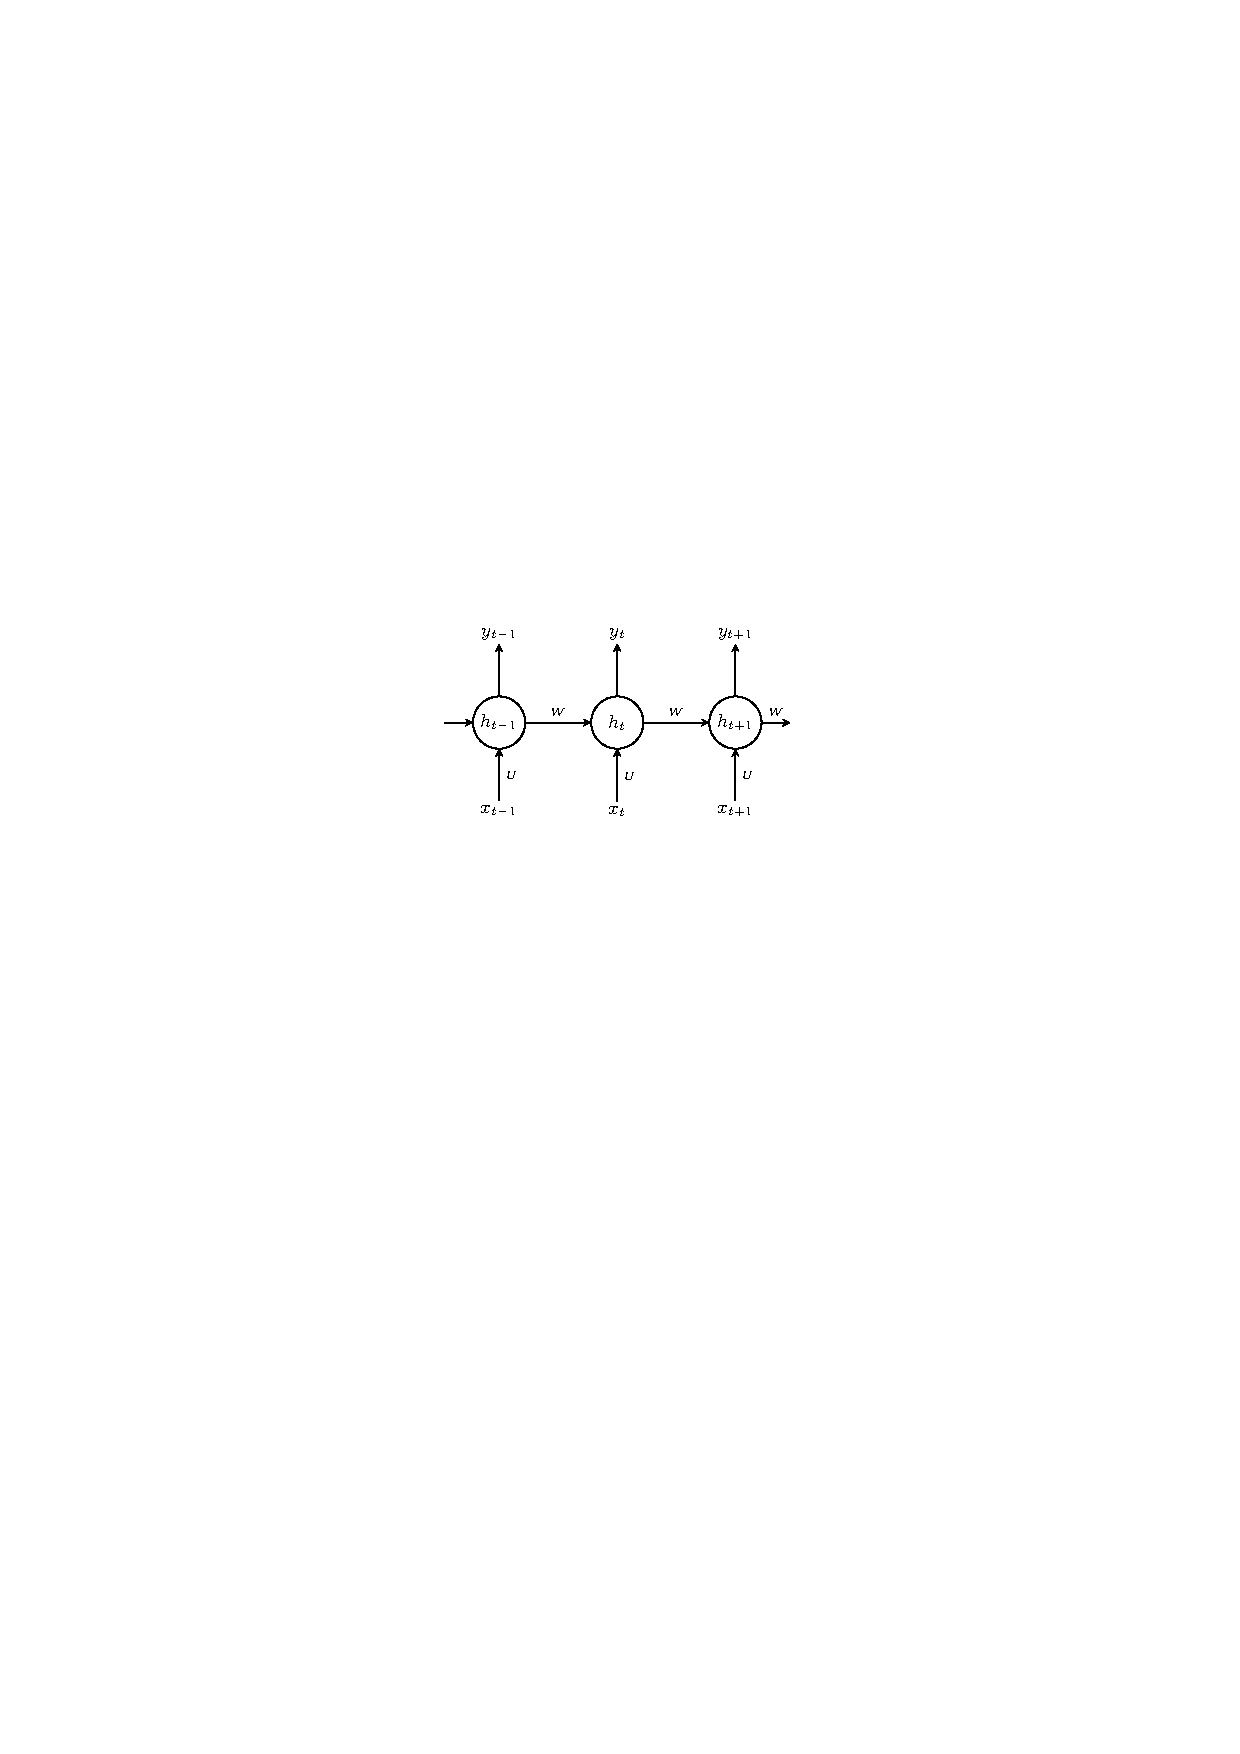
\includegraphics[scale=1.2]{rnn.pdf}
\vspace{-1em}
\caption{A recurrent neural network.}
\end{figure*}

\noindent Each state $h_t$ is given by:
\begin{equation*}
h_t = \sigma(W h_{t-1} + U x_t), \text{where } \sigma(z) =\frac{1}{1+\exp(-z)} \,.
\end{equation*}
Let $L$ be a loss function defined as the sum over the losses $L_t$ at every time step until time $T$: $L=\sum_{t=0}^T L_t$, where $L_t$ is a scalar loss depending on $h_t$.

In the following, we want to derive the gradient of this loss function with respect to the parameter $W$.

(a) Suppose we have $y=\sigma(Wx)$ where $y\in \mathbb{R}^n, x\in \mathbb{R}^d$ and $W \in \mathbb{R}^{n \times d}$. Derive the Jacobian $\frac{\partial y}{\partial x} = \mathrm{diag}(\sigma') W \in \mathbb{R}^{n \times d}$.\\

\textbf{\textcolor{ans}{Answer. $\frac{\partial y}{\partial x}=\frac{\partial\sigma(Wx)}{\partial x}=\frac{\partial \sigma(Wx)}{\partial (Wx)}\times \frac{\partial (Wx)}{\partial x}=\mathrm{diag}(\sigma')W$}.\\}

(b) Derive the quantity $\frac{\partial L}{\partial W} = \sum_{t=0}^T \sum_{k=1}^t \frac{\partial L_t}{\partial h_t} \frac{\partial h_t}{\partial h_k} \frac{\partial h_k}{\partial W}$. \\

\textbf{\textcolor{ans}{Answer. $\frac{\partial L}{\partial W}=\frac{\partial(\sum_{t=0}^T L_t)}{\partial W}=\sum_{t=0}^T (\frac{\partial L_t}{h_t}\times  \frac{\partial h_t}{\partial W})=\sum_{t=0}^T\sum_{k=0}^{t-1}(\frac{\partial L_t}{\partial h_t}\times \frac{\partial h_t}{\partial h_{t-k}}\times \frac{\partial h_{t-k}}{\partial W})=\sum_{t=0}^T\sum_{k=1}^{t}(\frac{\partial L_t}{\partial h_t}\times \frac{\partial h_t}{\partial h_{k}}\times \frac{\partial h_k}{\partial W})$}.\\}

\clearpage
\section{\begingroup \large Exercise 2: Vanishing/Exploding Gradients in RNNs \endgroup}

\noindent In this exercise, we want to understand why RNNs (Recurrent Neural Networks) are especially prone to the Vanishing/Exploding Gradients problem and what role the eigenvalues of the weight matrix play. Consider part (b) of exercise 1 again.

(a) Write down $\frac{\partial L}{\partial W}$ as expanded sum for $T = 3$. You should see that if we want to backpropagate through $n$ timesteps, we have to multiply the matrix $\mathrm{diag}(\sigma')W$ $n$ times with itself.\\

\textcolor{ans}{\textbf{Answer.} When $T=3$, $\frac{\partial L}{\partial W}=\sum_{t=0}^3\sum_{k=1}^{t}(\frac{\partial L_t}{\partial h_t}\times \frac{\partial h_t}{\partial h_{k}}\times \frac{\partial h_k}{\partial W})$. Considering $h_t=\sigma(Wh_{t-1}+U_{x_t})$,  $\frac{\partial h_t}{\partial h_{t-1}}=\mathrm{diag}(\sigma')W$. Hence that $\frac{\partial h_n}{\partial h_0}={[\mathrm{diag}(\sigma')W]}^n$ for back-propagating through n timesteps. Specifically, if back-propagate through 3 timesteps, $\frac{\partial h_n}{\partial h_0}={[\mathrm{diag}(\sigma')W]}^3$.}\\

(b) Remember that any diagonalizable (square) matrix $M$ can be represented by its eigendecomposition $M=Q\Lambda Q^{-1}$  where $Q$ is a matrix whose $i$-th column corresponds to the $i$-th eigenvector of $M$ and $\Lambda$ is a diagonal matrix with the corresponding eigenvalues placed on the diagonals. Recall that every eigenvector $v_i$ satisfies this linear equation $M v_i = \lambda_i v_i$, where $\lambda_i = \Lambda_{ii}$ is an eigenvalue of $M$. Proof by induction that for such a matrix the product $\prod_{i=1}^n M$ can be represented as: $M^n = Q \Lambda^n Q^{-1}$.\\

\textcolor{ans}{\textbf{Answer.} $M^n=(Q\Lambda Q^{-1})^n=\prod_{i=1}^n(Q\Lambda Q^{-1}) =Q\Lambda^nQ^{-1}$.}\\

(c) Consider the weight matrix $\begin{bmatrix} 0.58 & 0.24 \\ 0.24 & 0.72 \end{bmatrix}$. Its eigendecomposition is:
\begin{equation*}
W = Q \Lambda Q^{-1} = \begin{bmatrix} 0.8 & -0.6 \\ 0.6 & 0.8 \end{bmatrix} \begin{bmatrix} 0.4 & 0 \\ 0 & 0.9 \end{bmatrix} \begin{bmatrix} 0.8 & 0.6 \\ -0.6 & 0.8 \end{bmatrix}
\end{equation*}
Calculate $W^{30}$. What do you observe? What happens in general if the absolute value of all eigenvalues of $W$ is smaller than $1$? What happens if the absolute value of any eigenvalue of $W$ is larger than $1$? What if all eigenvalues are $1$?\\

\textcolor{ans}{\textbf{Answer.} $W^{30}=\begin{bmatrix} 0.015261 & -0.020348 \\ -0.020348 & 0.027130 \end{bmatrix}$. When absolutes of all $W$'s eigenvalues are all smaller than $1$, values in $W^{30}$ are pretty small, meaning the gradients are vanishing. While absolutes of all $W$'s eigenvalues are all larger than $1$, values in $W^{30}$ are relatively large. When absolutes of all $W$'s eigenvalues all equal to $1$, the diagonals of $W^{30}$ are 1.}\\

\clearpage
\section{\begingroup \large Exercise 3: LSTMs \endgroup}
 
 \noindent Recall the elements of a module in an LSTM and the corresponding computations, where $\odot$ stands for pointwise multiplication. For a good explanation on LSTMs you can refer to \url{https://colah.github.io/posts/2015-08-Understanding-LSTMs/}. Consider the LSTM in Figure~2.
\begin{figure*}[t]
\label{fig:lstms}
\centering
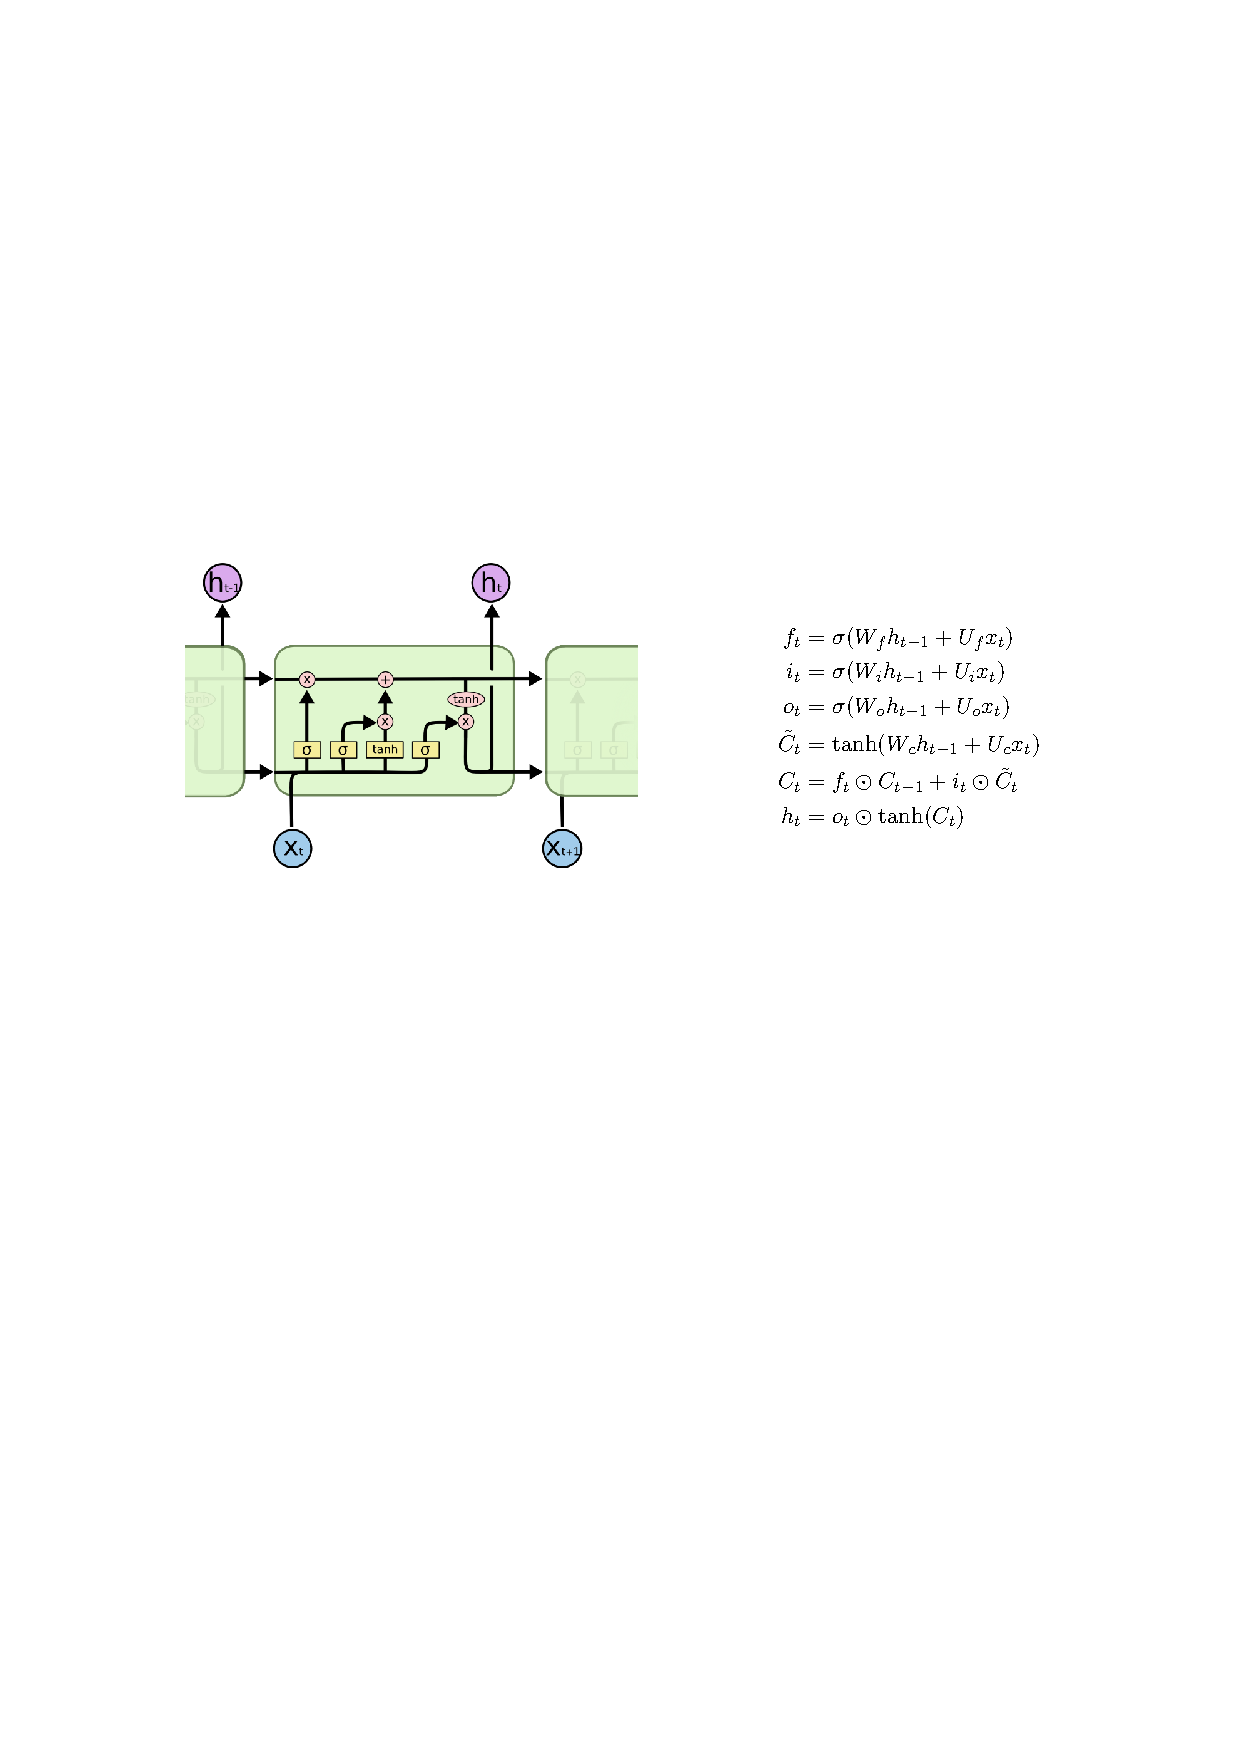
\includegraphics[scale=1.0]{lstm.pdf}
\vspace{-1em}
\caption{A Long Short Term Memory network.}
\end{figure*}
 
 (a) What do the gates $f_t$, $i_t$ and $o_t$ do? \\

\textcolor{ans}{\textbf{Answer.} $f_t$ is forget gate, deciding the reserving information. $i_t$ is input gate, deciding the updating information. $o_t$ is output gate, deciding the outputting information. \\}
 
 (b) Which of the quantities next to the figure are always positive? \\

\textcolor{ans}{\textbf{Answer.} Gate $f_t$, $i_t$, and $o_t$. This architecture tackles the gradient vanishing problem by the follows. To calculate $\frac{\partial L}{\partial \theta}$, where $\theta$ is ($W_f, W_o, W_i, W_c$), we need to consider $C_t$ as $h_t$ in RNN. Since $C_t$ depends on its previous state $C_{t-1}$, we have $\frac{\partial L}{\partial W}=\sum_{t=0}^T (\frac{\partial L_t}{h_t}\times  \frac{\partial h_t}{\partial W})=\sum_{t=0}^T\sum_{k=1}^{t}(\frac{\partial L_t}{\partial C_t}\times \frac{\partial C_t}{\partial C_{k}}\times \frac{\partial C_k}{\partial W})$.}

\textcolor{ans}{ \textit{Note that the real formula is more complicated, where we also need to take $f_t$, $i_t$, and $\tilde{C_t}$ into consideration. But the effect of these factors is negligible.} \\}
 
 \noindent Let’s now try to understand how this architecture approaches the vanishing gradients problem. To calculate the gradient $\frac{\partial L}{\partial \theta}$, where $\theta$ stands for the parameters $(W_f, W_o, W_i, W_c)$, we now have to consider the cell state $C_t$ instead of $h_t$. Like $h_t$ in normal RNNs, $C_t$ will also depend on the previous cell states $C_{t-1}, \ldots, C_0$, so we get a formula of the form:
 \begin{equation*}
 \frac{\partial L}{\partial W} = \sum_{t=0}^T \sum_{k=1}^t \frac{\partial L}{\partial C_t} \frac{\partial C_t}{\partial C_k} \frac{\partial C_k}{\partial W},
 \end{equation*}
 where note that the real formula is a bit more complicated since $C_t$ also depends on $f_t$, $i_t$ and $\widetilde{C}_t$, which in turn all depend on $W$, but this can be neglected.
 
 (c) We know that $\frac{\partial C_t}{\partial C_k} = \prod_{i=k+1}^t \frac{\partial C_t}{\partial C_{t-1}}$. Let $f_t=1$ and $i_t=0$ such that $C_t = C_{t-1}$ for all $t$. What is the gradient $\frac{\partial C_t}{\partial C_k}$ in this case?\\

\textcolor{ans}{\textbf{Answer.} When $f_t=1$ and $i_t=0$, $\frac{\partial C_t}{\partial C_k}=\prod_{i=k+1}^{t}\frac{\partial (f_i\odot C_{i-1}+i_i \odot \tilde{C_i})}{\partial C_{i-1}}=\prod_{i=k+1}^{t}\frac{\partial C_{i-1}}{\partial C_{i-1}}=1$.}

\clearpage
\section{\begingroup \large Acknowledgements \endgroup}

\noindent \begin{itemize} \item{First and foremost, I would like to show my deepest gratitude to my teacher, \textbf{Shangsong Liang}, who has provided us with valuable theoretical guidance of deep learning. Without his enlightening instruction, impressive kindness and patience, I could never have completed our homework. His keen and vigorous academic observation enlightens me in this thesis and my future study.}
\item{My sincere appreciation also goes to my \textbf{classmates}. We got along in harmony, discussed tasks together, and they gave me valuable advice. All of these make this experience meaningful.}
\end{itemize}

\end{document}